%
% Usability-Evaluierungen mit der thEvaluator-Applikation
% Abschlussarbeit (Bachelor)
%
% Thema: Erstellung einer Browser Extension zur Usability Evaluierung von beliebigen Web-Applikationen über Heatmaps.
% Betreuer 1: Prof. Dr. Targo Pavlista
% Betreuer 2: Siamak Haschemi
%
% @author Christian Bromann <contact@christian-bromann.com>
%

\chapter{Usability-Evaluierungen mit der thEvaluator-Applikation}

% TODO write sth...

%
% Evaluierung der Beuth-Hochschulseite
% Abschlussarbeit (Bachelor)
%
% Thema: Erstellung einer Browser Extension zur Usability Evaluierung von beliebigen Web-Applikationen über Heatmaps.
% Betreuer 1: Prof. Dr. Targo Pavlista
% Betreuer 2: Siamak Haschemi
%
% @author Christian Bromann <contact@christian-bromann.com>
%

\section{Evaluierung der Beuth-Hochschulseite}

Hochschulseiten, wie die der Beuth-Hochschule, gelten als reine Informationsseiten und haben es schwer, den vielen Inhalt möglichst benutzerfreundlich an den User zu bringen. Wie in Kapitel \ref{usability-auf-uniseiten} bereits thematisiert, muss die Seite den Anforderungen vieler verschiedener Menschen aufkommen, die den Service jeweils mit unterschiedlicher Erfahrung nutzen. Der Test soll zeigen, wie der Nutzer auf der Seite navigiert und wie schnell er dabei die gesuchten Informationen findet.

\subsection{Simuliertes Szenario}

Der Tescase ist in Form einer Geschichte aufgebaut. Diese soll den Probanden in die Lage eines frisch absolvierten Abiturienten versetzen, der nach seinem Abschluss auf der Suche nach einem Studiengang an der Beuth Hochschule ist. Der Proband wird konfrontiert mit Aufgaben, mit denen der Abiturient ebenfalls zu tun hätte. Neben dem Öffnen des Modulhandbuches oder das Informieren über bestimmte Fristen muss der User ebenfalls die Online-Bewerbung starten oder sich in Kurse einschreiben. Hier wird es interessant zu beobachten sein, welchen Weg der Nutzer einschlägt, um an sein Ziel zu gelangen.

\subsection{Auswertung der Daten}

Die erste wichtige Erkenntnis, die die Auswertung der Daten erbringt, ist die häufige Nutzung der Suchfunktion der Seite. Viele Heat- und Clickmaps zeigen, wie die Nutzer auf das Eingabefeld der Suche klicken, anstatt sich durch die Navigationsbäume zu hangeln. Ein Ausschnitt der Clickmap von der Startseite (Bild \ref{clickmapSearch}) zeigt, wie wichtig dieses Element für die Suche nach speziellen Informationen ist.
\\
\begin{center}
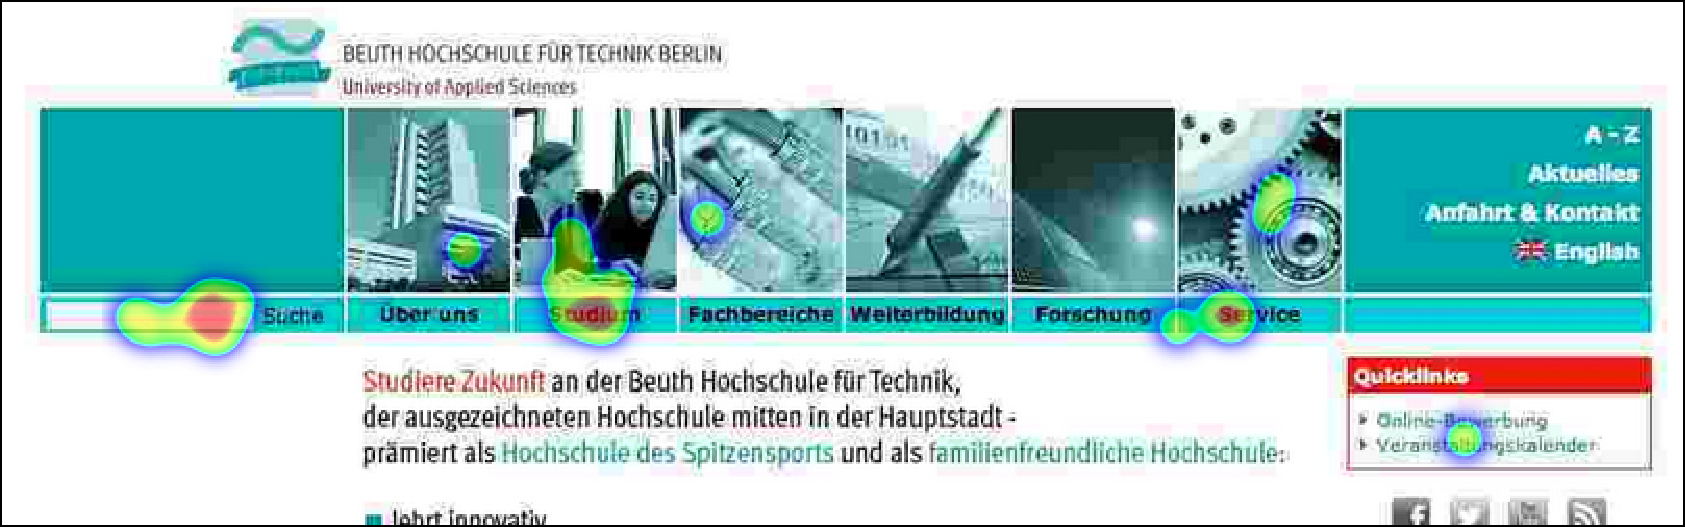
\includegraphics[scale=0.52]{./images/clickmap-search}
\end{center}
\begin{figure}[htb]
   \centering
   \caption{Clickmap der Startseite (Ausschnitt)}
    \label{clickmapSearch}
\end{figure}

Auch in den Verlaufspfaden der Besucher ist oft die Seite der Suchresultate zu finden. In ca. 75\% der Fälle wird, entweder direkt oder auf der nachfolgenden Seite, die gesuchte Information gefunden und die Aufgabe gelöst. Folgender User-Kommentar bestätigt zusätzlich diese Annahme. In dem hieß es:

\begin{quote}
     \glqq \textit{Ich konnte mich nicht so gut in einen Studenten versetzen. Statt [...] auf der Website zu navigieren und zu lesen, habe ich öfter die Suche, die recht eindeutige Ergebnisse ausgab, benutzt.}\grqq{}
\end{quote}

Die Suche erwies sich also für viele als sehr hilfreich und scheint in den meisten Fällen auch zum Erfolg zu führen. Positiv anzumerken ist hier, dass sie auf fast jeder Seite immer recht prominent an der selben Stelle zu finden ist. So muss der Nutzer nicht lange suchen, um auf sie zuzugreifen. Dennoch könnte sie mehr hervorgehoben werden, da das kleine Eingabekästchen nicht den Eindruck erweckt, sehr funktionsreich zu sein.\\
\\
Wie wichtig eine feste Position von wichtigen Seitenelementen ist, zeigt die nächste Beobachtung. Der Aufbau der Beuth-Seite ist sehr strikt gehalten und zieht sich auf fast allen Seiten durch. Ganz oben ist das Logo (links/mitte) platziert gefolgt von der Hauptnavigation. Im unteren Teil der Seite befindet sich der Content (mittig), umrahmt von der Subnavigation (links und rechts). Im Gegensatz dazu besitzen die Seiten einiger Fachbereiche ein ganz anderes Design. Dies ist jedoch weiter nicht schlimm, da das Aussehen und der Aufbau sich soweit unterscheiden, dass der User sich sofort neu orientiert, wenn er über ein Link von der Beuth-Seite kommt. Auf den Informationsseiten über Professoren\footnote{\url{http://prof.beuth-hochschule.de}}, Projekte\footnote{\url{http://labor.beuth-hochschule.de}} oder Labore\footnote{\url{http://projekt.beuth-hochschule.de}} der Beuth Hochschule ist dies leider nicht der Fall. Das Aussehen ähnelt hier stark dem der Hauptseite, unterscheidet sich jedoch im Aufbau bei wichtigen Seitenelementen. Die Hauptnavigation fällt dort komplett raus, das Suchelement ist entfernt und das Logo ist auf die rechte Seite gerutscht. Es bleiben lediglich die gekachelten Bilder und die Subnavigation, die den Content umrahmt. Folgt der Benutzer einen Link auf diese Seite, so ist ihm im ersten Moment nicht bewusst, dass diese anders aufgebaut ist. Fixe Navigationselemente werden an gleicher Stelle erwartet wie auf den vorherigen Seiten. Geht der User nun mit der Maus zur Position, wo er das Logo, die Suche oder die Hauptnavigation erwartet, so stellt er fest, dass diese verschwunden sind. Aufgrund der Orientierungslosigkeit ist er gezwungen die Seite noch einmal mit seinen Augen komplett neu abzuscannen, um herauszufinden, wie es weiter geht. Abbildung \ref{heatmapPavlista} zeigt dieses Verhalten recht deutlich.

\begin{center}
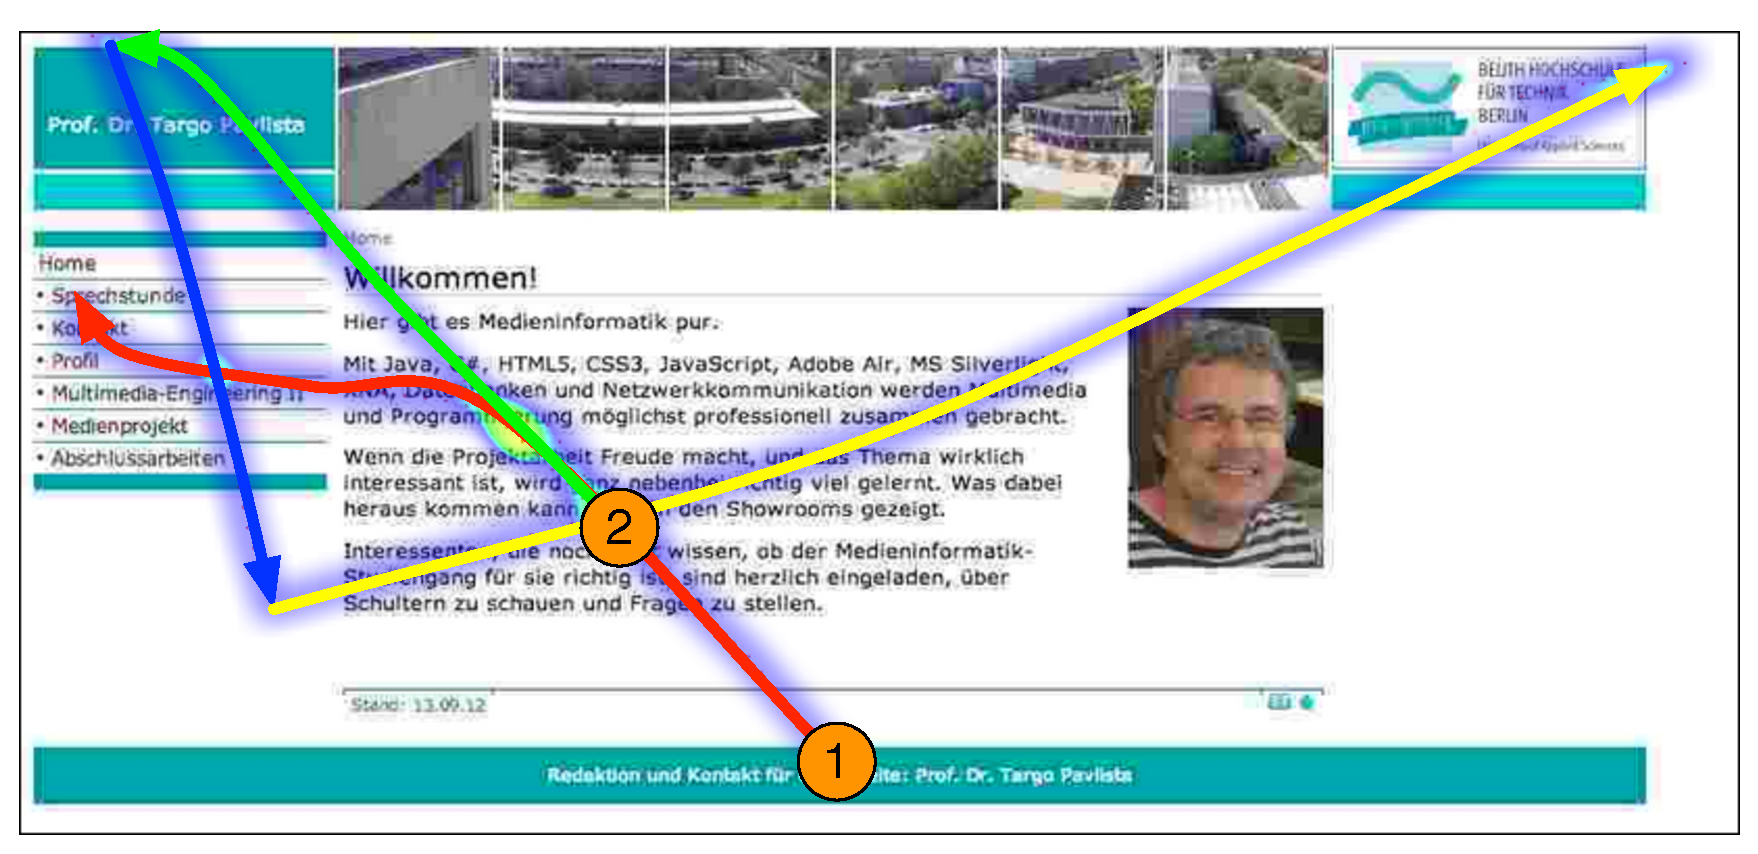
\includegraphics[scale=0.52]{./images/heatmapPavlista}
\end{center}
\begin{figure}[htb]
   \centering
   \caption{Bewegungsverlauf der Maus auf der Suche nach dem Link zur Startseite}
    \label{heatmapPavlista}
\end{figure}

Der Nutzer startete am Punkt 1 (\textbf{{\color{orange}oranger}} Kreis). Seine Aufgabe war es, die Sprechzeiten von Prof. Dr. Targo Pavlista zu finden. Diese Aufgabe ist erledigt mit dem Klick auf den Link \glqq Sprechstunde\grqq{} in der Subnavigation (vgl. \textbf{{\color{red}roter}} Pfeil). Daraufhin blendete das Tool den Popup mit der Beschreibung der nächsten Aufgabe ein. Dieses bestätigte der User und befand sich anschließend an Punkt 2. Die erste intuitive Aktion war es nun auf das Logo zu klicken, um zurück zur Startseite zu gelangen (vgl. \textbf{{\color{green}grüner}} Pfeil). Dieses wurde an der gewohnten Position (oben links) erwartet, doch nicht gefunden. Daraufhin musste die Seite neu abgescannt werden, um einen Überblick über den Aufbau zu erhalten (vgl. \textbf{{\color{blue}blauer}} Pfeil). Nachdem dies geschah und die neue Position des Logos mit dem Link zur Startseite gefunden wurde, bewegte sich die Maus dorthin und der User verlies die Seite (vgl. \textbf{{\color{yellow}gelber}} Pfeil). Dieses Verhalten bestätigen auch Heatmaps anderer Testläufe. Teilweise wurde das Bild mit dem Logo auf der rechten Seite gar nicht als Link zur Startseite erkannt. Die Nutzer mussten daraufhin die URL der Seite neu eingeben, um dorthin zu gelangen. Das Beispiel zeigt, wie wichtig es ist, die Struktur der Seite beizubehalten und an eine feste Position für wichtige Elemente, wie z.B. Logo oder Navigation, festzuhalten. Der User gewöhnt sich schnell an eine vorgegebene Seitenstruktur. Sein Besuch wird gestört, wenn diese sich ändert und er gezwungen ist, sich neu zu orientieren.\\
\\
Die meisten Webseiten erstrecken sich bei viel Inhalt auf der y-Achse. Dies führt dazu, dass der Nutzer scrollen muss, um den ganzen Inhalt erfassen zu können. Handelt es sich dabei um Text, so wird dies nicht als störend empfunden, da der User so in seinem Lesefluss bleibt. Bei einer langen Liste von Einträgen, wie z.B. bei Aufzählungen, kann dies jedoch zu Usability-Problemen führen. Der Nutzer verliert durch das Scrollen die Übersicht und damit die Orientierung auf der Seite. Ihm fällt es dadurch schwerer, einen bestimmten Eintrag aus der Liste zu finden.\\
In einer der Aufgaben des Testcases muss der User das Modulhandbuch des Studiengangs \textit{Medieninformatik} öffnen. Der Link dazu befindet sich auf dessen Informationsseite. Um dahin zu gelangen, kann der Nutzer entweder die Suche nutzen oder den Link dorthin aus einer langen Liste aller Studienangebote der Hochschule finden. Viele User, die sich für den letzten Weg entschieden haben, brauchten deutlich mehr Zeit zum Lösen der Aufgabe. Grund dafür ist die benutzerunfreundliche Gestaltung der Liste. Wie Abbildung \ref{gazeplotCourses} zeigt, scannen die User teilweise die gesamte Liste ab, um den gesuchten Eintrag (in \textbf{{\color{magenta}magenta}} hervorgehoben) zu finden. Neben den Mausbewegungen sind ebenfalls die Stellen, in Form von blauen Kreisen, markiert, an denen sich die Maus für eine gewisse Zeit nicht bewegt hat. Wie bereits in Kapitel \ref{metrics} erläutert, ist die Größe des Kreises ein Maß dafür, wie lange sich die Maus im Mittelpunkt aufgehalten hat.

\begin{center}
\frame{\includegraphics[scale=0.205]{./images/gazeplotCourses}}
\end{center}
\begin{figure}[htb]
   \centering
   \caption{Gazeplot Auswertung der Beuth-Seite mit der Liste aller Studienangebote}
    \label{gazeplotCourses}
\end{figure}

Je größer der Kreis ist, desto länger hat sich die Maus nicht bewegt. Wie in der Abbildung zu erkennen ist, sind viele Kreise in der unteren Hälfte der Seite zu finden. Viele User haben beim Scrollen den gesuchten Eintrag nicht wahrgenommen und sind zum Schluss am Ende der Seite angelangt. Nach einer kurzen Zeit der Neuorientierung, mussten sie wieder aufwärts scrollen, um den Eintrag zu finden. Dies kostet dem User Zeit und Geduld.\\
Auf vielen Seiten, oft sogar mit noch längeren Listen, ist dieses Problem ebenfalls zu beobachten. Schon durch einfache Methoden kann die Benutzerfreundlichkeit dieser schnell verbessert werden. Sprungmarken bspw. geben dem User die Möglichkeit, zu einer bestimmten Stelle in der Liste zu \glqq springen\grqq{}. Ist die Liste, wie in diesem Beispiel, von A bis Z geordnet, so bestehen die Sprungmarken aus den Buchstaben des Alphabetes und führen zum ersten Eintrag, welcher mit dem jeweiligen Buchstaben beginnt. Eine etwas aufwendigere Lösung, die jedoch bei größeren Listen besser geeignet ist, wäre die Nutzung einer Filterbox. Der User kann damit durch Eingabe eines Suchstrings die Liste filtern. Ohne die Seite neu zu laden wird nach jeder Eingabe eines Buchstaben die Einträge, die nicht mit dem Suchstring übereinstimmen, aus der Liste entfernt. Dadurch findet der User schon nach wenigen Buchstaben eine stark dezimierte Liste, aus der der gewünschte Eintrag benutzerfreundlich ausgewählt werden kann.\\
\\
Alles in Allem ist die Auswertung der Usability der Hochschulseite besser ausgefallen als erwartet. Mehr als die Hälfte der Probanden konnte den Testcase erfolgreich lösen. Die Zeit, die dafür gebraucht wurde, war jedoch recht lang. Der längste Testlauf lief ca. 16 Minuten und entspricht dem 5-fachen der Zeit, die jemand benötigt, wenn er die Seite bereits kennt. Aufgefallen ist ebenfalls die häufige Nutzung der Suche, die zu relativ zufriedenstellenden Ergebnissen führt. Nichtsdestotrotz sind Mithilfe des Tools ein paar Problemstellen gefunden worden, die den User beim Besuchen der Webseite stören könnte. Die folgende Tabelle gibt noch einmal einen kurzen Überblick über das Ergebnis des Tests.\\
\\
\begin{center}
{\footnotesize
\begin{tabular}{ p{6.5cm} p{1.2cm} }
  \hline
  Anzahl der Teilnehmer &13\vspace{0.2cm}\\
  Erfolgreich abgeschlossene Testläufe & 7\vspace{0.2cm}\\
  Abgeschlossene Testläufe durch Timeout & 3\vspace{0.2cm}\\
  Abgebrochene Testläufe & 3\vspace{0.2cm}\\
  Durchschnittliche Dauer eines Tests & 11,3 min\\
  \hline
\end{tabular}
}
\vspace{0.3cm}
\captionof{table}{Ergebnisse des Tests als Übersicht} \label{tab:title}
\vspace{0.3cm}
\end{center}











%
% Evaluierung der thEvaluator-Applikation
% Abschlussarbeit (Bachelor)
%
% Thema: Erstellung einer Browser Extension zur Usability Evaluierung von beliebigen Web-Applikationen über Heatmaps.
% Betreuer 1: Prof. Dr. Targo Pavlista
% Betreuer 2: Siamak Haschemi
%
% @author Christian Bromann <contact@christian-bromann.com>
%

\section{Evaluierung der thEvaluator-Applikation}

Nach vielen Wochen der selbstständigen und alleinigen Entwicklung an einem Tool ist schnell das richtige Gefühl über die Qualität des Gesamtproduktes verloren. Als Entwickler befindet man sich in einer Art Tunnel und übersieht schnell Probleme, die eine fremde Person auf anhieb finden würde. Aus diesem Grund war es wichtig, die Applikation zu testen, um herauszufinden, ob auch andere Personen das Tool richtig benutzen können.

\subsection{Simuliertes Szenario}

In den Aufgaben im Test ging es vor allem darum, einen Testcase selber zu erstellen und die Funktionen der Seite kennenzulernen. Es war interessant zu sehen, welche Daten der Proband in die Formulare eingetragen hat. Daraus lies sich schnell erschließen, ob dieser mit den Anforderungen vertraut war oder nicht wusste was er auszufüllen hatte. Besondere Aufmerksamkeit galt dem Task-Formular. Eine Aufgabe sah es vor, einen Task zu erstellen, dessen Ziel der Klick auf einen Link vorsieht. Eine Erklärung zur Definition einer Ziel-Action wurde weder in der Email an die Probanden noch in der Aufgabenstellung mitgegeben. Hier war somit nicht zu erwarten, dass sich die Benutzer richtig verhalten.

\subsection{Auswertung der Daten}

Nach Auswertung der Daten dieses Tests bestätigten sich die Vermutungen aus dem letzten Absatz. Die Probanden waren nicht immer in der Lage, immer die richtigen Daten in das Formular einzutragen. Gerade beim Task-Formular hat es schwerwiegende Probleme gegeben. Kein User hat es geschafft einen Task nach den Vorgaben der Aufgabe zu erstellen. Hauptursache dafür ist möglicherweise die mangelnde Beschreibung des Zielaktions-Feldes. In einem Testcase füllte ein Proband das Feld mit den Worten: \glqq \textit{versteh ich nicht}\grqq{} aus. Höchstwahrscheinlich war es die selbe Person, die am Ende den folgenden Text in der Feedbackbox hinterließ:

\begin{quote}
     \glqq \textit{Konnte nicht mit allen Eingabeaufforderungen was anfangen.
    Wieso Cookie? Und die Auswahlmöglichkeit mit Blur, usw hab ich auch nicht gecheckt}\grqq{}
\end{quote}

Wie in Kapitel \ref{targetElem} beschrieben verlangt das Zielaktions-Feld die Eingabe eines Query-Selektors aus dem DOM der Seite. Die User hätten lediglich das Feld mit einem \glqq \textit{a}\grqq{} befüllen müssen, da keine genauen Angaben über den Link genannt wurden. Als Aktion wäre \glqq \textit{click}\grqq{} richtig gewesen. Da es keinerlei Beschreibung für dieses Feld gab und die Probanden kaum Erfahrungen in Umgang mit Selektoren in einer HTML Seite hatten, ist das Resultat gut nachvollziehbar. Die nachfolgende Tabelle fasst noch mal kurz das Ergebnis des Tests zusammen.
\\
\begin{center}
{\footnotesize
\begin{tabular}{ p{6.5cm} p{1.1cm} }
  \hline
  Anzahl der Teilnehmer & 5\vspace{0.2cm}\\
  Erfolgreich abgeschlossene Testläufe & 2\vspace{0.2cm}\\
  Abgeschlossene Testläufe durch Timeout & 2\vspace{0.2cm}\\
  Abgebrochene Testläufe & 1\vspace{0.2cm}\\
  Durchschnittliche Dauer eines Tests & 8,2 min\\
  \hline
\end{tabular}
}
\vspace{0.3cm}
\captionof{table}{Ergebnisse des Test als Übersicht} \label{tab:title}
\vspace{0.3cm}
\end{center}

Die Tatsache, dass bei zwei Testläufen die Zeit abgelaufen ist, lässt vermuten, dass der User zu lange zum Ausfüllen der Formulare gebraucht hat. Dies wird auch durch Einen der Feedback-Texte bestätigt. Darin hieß es: \glqq \textit{Puh! Wenig Zeit gehabt. [...]}\grqq{}. Aus Usability-Sicht könnten hier Hinweis-Links helfen, die dem Besucher Hilfestellung geben.
%
% Usability-Evaluierungen mit der thEvaluator-Applikation
% Abschlussarbeit (Bachelor)
%
% Thema: Erstellung einer Browser Extension zur Usability Evaluierung von beliebigen Web-Applikationen über Heatmaps.
% Betreuer 1: Prof. Dr. Targo Pavlista
% Betreuer 2: Siamak Haschemi
%
% @author Christian Bromann <contact@christian-bromann.com>
%

\chapter{Usability-Evaluierungen mit der thEvaluator-Applikation}

% TODO write sth...

%
% Evaluierung der Beuth-Hochschulseite
% Abschlussarbeit (Bachelor)
%
% Thema: Erstellung einer Browser Extension zur Usability Evaluierung von beliebigen Web-Applikationen über Heatmaps.
% Betreuer 1: Prof. Dr. Targo Pavlista
% Betreuer 2: Siamak Haschemi
%
% @author Christian Bromann <contact@christian-bromann.com>
%

\section{Evaluierung der Beuth-Hochschulseite}

Hochschulseiten, wie die der Beuth-Hochschule, gelten als reine Informationsseiten und haben es schwer, den vielen Inhalt möglichst benutzerfreundlich an den User zu bringen. Wie in Kapitel \ref{usability-auf-uniseiten} bereits thematisiert, muss die Seite den Anforderungen vieler verschiedener Menschen aufkommen, die den Service jeweils mit unterschiedlicher Erfahrung nutzen. Der Test soll zeigen, wie der Nutzer auf der Seite navigiert und wie schnell er dabei die gesuchten Informationen findet.

\subsection{Simuliertes Szenario}

Der Tescase ist in Form einer Geschichte aufgebaut. Diese soll den Probanden in die Lage eines frisch absolvierten Abiturienten versetzen, der nach seinem Abschluss auf der Suche nach einem Studiengang an der Beuth Hochschule ist. Der Proband wird konfrontiert mit Aufgaben, mit denen der Abiturient ebenfalls zu tun hätte. Neben dem Öffnen des Modulhandbuches oder das Informieren über bestimmte Fristen muss der User ebenfalls die Online-Bewerbung starten oder sich in Kurse einschreiben. Hier wird es interessant zu beobachten sein, welchen Weg der Nutzer einschlägt, um an sein Ziel zu gelangen.

\subsection{Auswertung der Daten}

Die erste wichtige Erkenntnis, die die Auswertung der Daten erbringt, ist die häufige Nutzung der Suchfunktion der Seite. Viele Heat- und Clickmaps zeigen, wie die Nutzer auf das Eingabefeld der Suche klicken, anstatt sich durch die Navigationsbäume zu hangeln. Ein Ausschnitt der Clickmap von der Startseite (Bild \ref{clickmapSearch}) zeigt, wie wichtig dieses Element für die Suche nach speziellen Informationen ist.
\\
\begin{center}
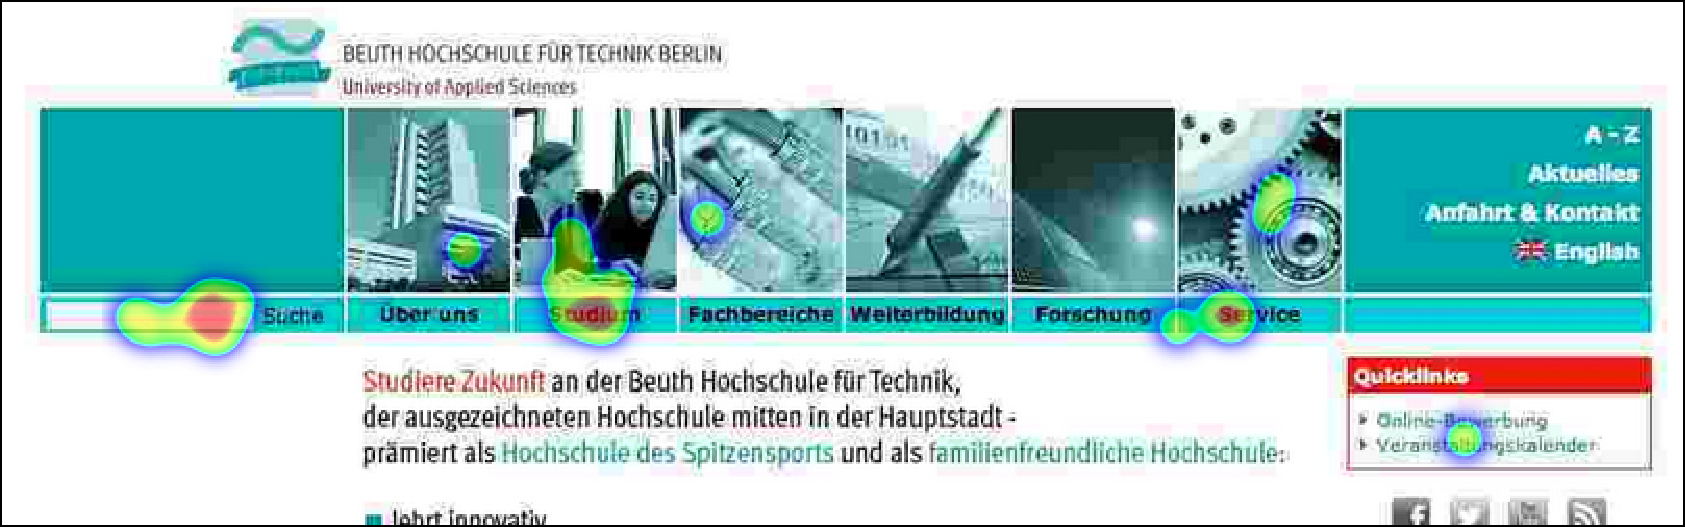
\includegraphics[scale=0.52]{./images/clickmap-search}
\end{center}
\begin{figure}[htb]
   \centering
   \caption{Clickmap der Startseite (Ausschnitt)}
    \label{clickmapSearch}
\end{figure}

Auch in den Verlaufspfaden der Besucher ist oft die Seite der Suchresultate zu finden. In ca. 75\% der Fälle wird, entweder direkt oder auf der nachfolgenden Seite, die gesuchte Information gefunden und die Aufgabe gelöst. Folgender User-Kommentar bestätigt zusätzlich diese Annahme. In dem hieß es:

\begin{quote}
     \glqq \textit{Ich konnte mich nicht so gut in einen Studenten versetzen. Statt [...] auf der Website zu navigieren und zu lesen, habe ich öfter die Suche, die recht eindeutige Ergebnisse ausgab, benutzt.}\grqq{}
\end{quote}

Die Suche erwies sich also für viele als sehr hilfreich und scheint in den meisten Fällen auch zum Erfolg zu führen. Positiv anzumerken ist hier, dass sie auf fast jeder Seite immer recht prominent an der selben Stelle zu finden ist. So muss der Nutzer nicht lange suchen, um auf sie zuzugreifen. Dennoch könnte sie mehr hervorgehoben werden, da das kleine Eingabekästchen nicht den Eindruck erweckt, sehr funktionsreich zu sein.\\
\\
Wie wichtig eine feste Position von wichtigen Seitenelementen ist, zeigt die nächste Beobachtung. Der Aufbau der Beuth-Seite ist sehr strikt gehalten und zieht sich auf fast allen Seiten durch. Ganz oben ist das Logo (links/mitte) platziert gefolgt von der Hauptnavigation. Im unteren Teil der Seite befindet sich der Content (mittig), umrahmt von der Subnavigation (links und rechts). Im Gegensatz dazu besitzen die Seiten einiger Fachbereiche ein ganz anderes Design. Dies ist jedoch weiter nicht schlimm, da das Aussehen und der Aufbau sich soweit unterscheiden, dass der User sich sofort neu orientiert, wenn er über ein Link von der Beuth-Seite kommt. Auf den Informationsseiten über Professoren\footnote{\url{http://prof.beuth-hochschule.de}}, Projekte\footnote{\url{http://labor.beuth-hochschule.de}} oder Labore\footnote{\url{http://projekt.beuth-hochschule.de}} der Beuth Hochschule ist dies leider nicht der Fall. Das Aussehen ähnelt hier stark dem der Hauptseite, unterscheidet sich jedoch im Aufbau bei wichtigen Seitenelementen. Die Hauptnavigation fällt dort komplett raus, das Suchelement ist entfernt und das Logo ist auf die rechte Seite gerutscht. Es bleiben lediglich die gekachelten Bilder und die Subnavigation, die den Content umrahmt. Folgt der Benutzer einen Link auf diese Seite, so ist ihm im ersten Moment nicht bewusst, dass diese anders aufgebaut ist. Fixe Navigationselemente werden an gleicher Stelle erwartet wie auf den vorherigen Seiten. Geht der User nun mit der Maus zur Position, wo er das Logo, die Suche oder die Hauptnavigation erwartet, so stellt er fest, dass diese verschwunden sind. Aufgrund der Orientierungslosigkeit ist er gezwungen die Seite noch einmal mit seinen Augen komplett neu abzuscannen, um herauszufinden, wie es weiter geht. Abbildung \ref{heatmapPavlista} zeigt dieses Verhalten recht deutlich.

\begin{center}
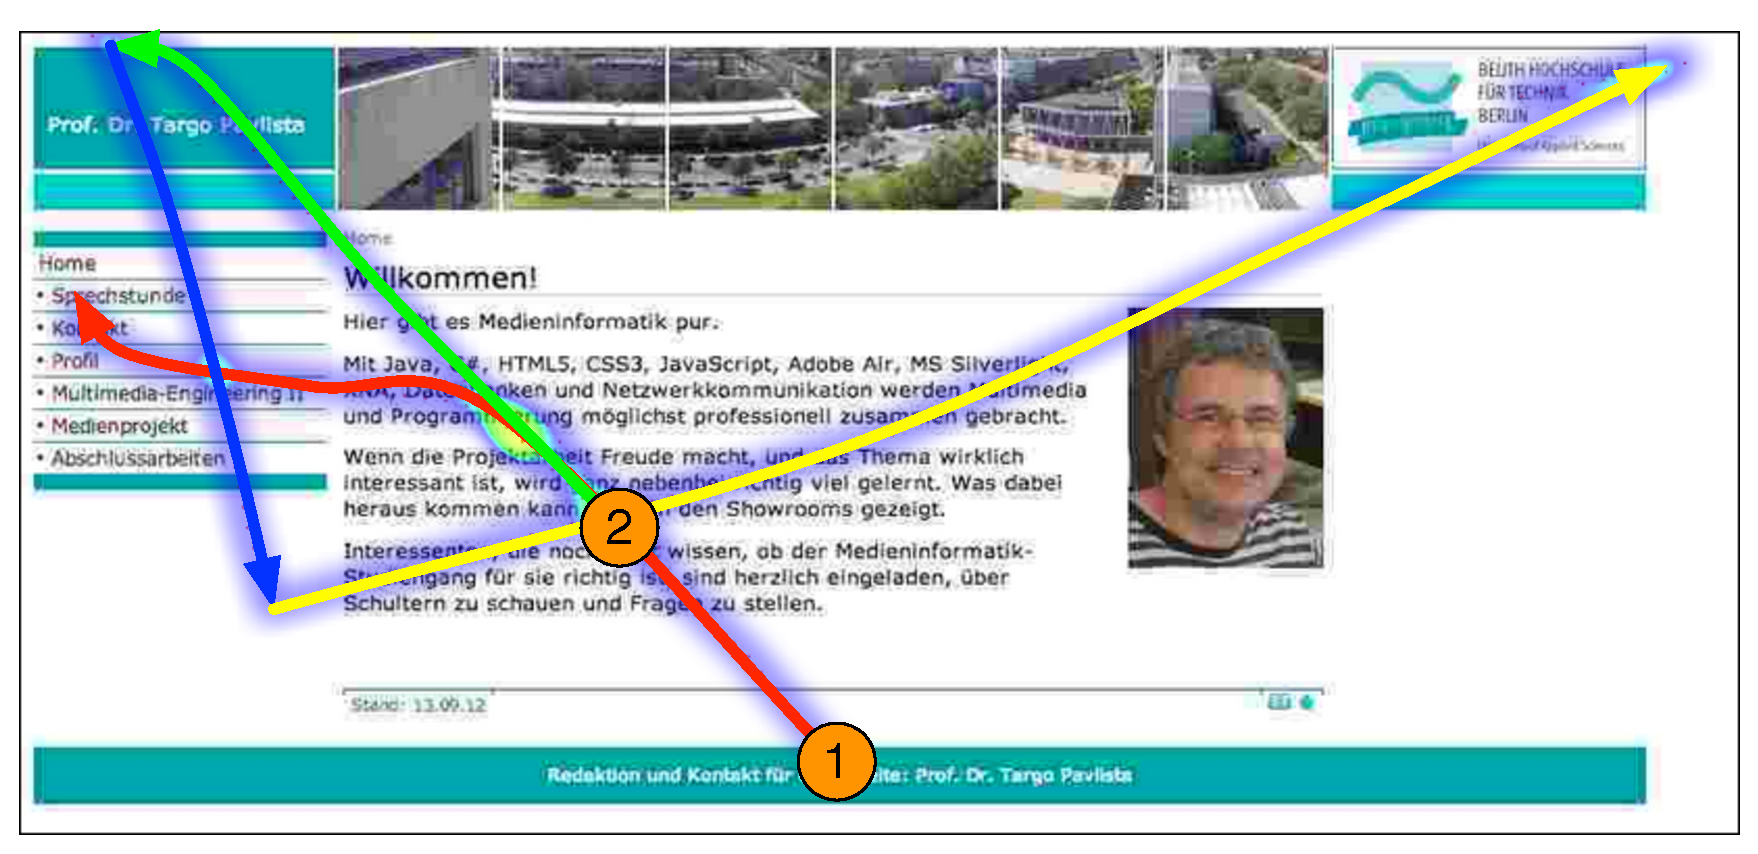
\includegraphics[scale=0.52]{./images/heatmapPavlista}
\end{center}
\begin{figure}[htb]
   \centering
   \caption{Bewegungsverlauf der Maus auf der Suche nach dem Link zur Startseite}
    \label{heatmapPavlista}
\end{figure}

Der Nutzer startete am Punkt 1 (\textbf{{\color{orange}oranger}} Kreis). Seine Aufgabe war es, die Sprechzeiten von Prof. Dr. Targo Pavlista zu finden. Diese Aufgabe ist erledigt mit dem Klick auf den Link \glqq Sprechstunde\grqq{} in der Subnavigation (vgl. \textbf{{\color{red}roter}} Pfeil). Daraufhin blendete das Tool den Popup mit der Beschreibung der nächsten Aufgabe ein. Dieses bestätigte der User und befand sich anschließend an Punkt 2. Die erste intuitive Aktion war es nun auf das Logo zu klicken, um zurück zur Startseite zu gelangen (vgl. \textbf{{\color{green}grüner}} Pfeil). Dieses wurde an der gewohnten Position (oben links) erwartet, doch nicht gefunden. Daraufhin musste die Seite neu abgescannt werden, um einen Überblick über den Aufbau zu erhalten (vgl. \textbf{{\color{blue}blauer}} Pfeil). Nachdem dies geschah und die neue Position des Logos mit dem Link zur Startseite gefunden wurde, bewegte sich die Maus dorthin und der User verlies die Seite (vgl. \textbf{{\color{yellow}gelber}} Pfeil). Dieses Verhalten bestätigen auch Heatmaps anderer Testläufe. Teilweise wurde das Bild mit dem Logo auf der rechten Seite gar nicht als Link zur Startseite erkannt. Die Nutzer mussten daraufhin die URL der Seite neu eingeben, um dorthin zu gelangen. Das Beispiel zeigt, wie wichtig es ist, die Struktur der Seite beizubehalten und an eine feste Position für wichtige Elemente, wie z.B. Logo oder Navigation, festzuhalten. Der User gewöhnt sich schnell an eine vorgegebene Seitenstruktur. Sein Besuch wird gestört, wenn diese sich ändert und er gezwungen ist, sich neu zu orientieren.\\
\\
Die meisten Webseiten erstrecken sich bei viel Inhalt auf der y-Achse. Dies führt dazu, dass der Nutzer scrollen muss, um den ganzen Inhalt erfassen zu können. Handelt es sich dabei um Text, so wird dies nicht als störend empfunden, da der User so in seinem Lesefluss bleibt. Bei einer langen Liste von Einträgen, wie z.B. bei Aufzählungen, kann dies jedoch zu Usability-Problemen führen. Der Nutzer verliert durch das Scrollen die Übersicht und damit die Orientierung auf der Seite. Ihm fällt es dadurch schwerer, einen bestimmten Eintrag aus der Liste zu finden.\\
In einer der Aufgaben des Testcases muss der User das Modulhandbuch des Studiengangs \textit{Medieninformatik} öffnen. Der Link dazu befindet sich auf dessen Informationsseite. Um dahin zu gelangen, kann der Nutzer entweder die Suche nutzen oder den Link dorthin aus einer langen Liste aller Studienangebote der Hochschule finden. Viele User, die sich für den letzten Weg entschieden haben, brauchten deutlich mehr Zeit zum Lösen der Aufgabe. Grund dafür ist die benutzerunfreundliche Gestaltung der Liste. Wie Abbildung \ref{gazeplotCourses} zeigt, scannen die User teilweise die gesamte Liste ab, um den gesuchten Eintrag (in \textbf{{\color{magenta}magenta}} hervorgehoben) zu finden. Neben den Mausbewegungen sind ebenfalls die Stellen, in Form von blauen Kreisen, markiert, an denen sich die Maus für eine gewisse Zeit nicht bewegt hat. Wie bereits in Kapitel \ref{metrics} erläutert, ist die Größe des Kreises ein Maß dafür, wie lange sich die Maus im Mittelpunkt aufgehalten hat.

\begin{center}
\frame{\includegraphics[scale=0.205]{./images/gazeplotCourses}}
\end{center}
\begin{figure}[htb]
   \centering
   \caption{Gazeplot Auswertung der Beuth-Seite mit der Liste aller Studienangebote}
    \label{gazeplotCourses}
\end{figure}

Je größer der Kreis ist, desto länger hat sich die Maus nicht bewegt. Wie in der Abbildung zu erkennen ist, sind viele Kreise in der unteren Hälfte der Seite zu finden. Viele User haben beim Scrollen den gesuchten Eintrag nicht wahrgenommen und sind zum Schluss am Ende der Seite angelangt. Nach einer kurzen Zeit der Neuorientierung, mussten sie wieder aufwärts scrollen, um den Eintrag zu finden. Dies kostet dem User Zeit und Geduld.\\
Auf vielen Seiten, oft sogar mit noch längeren Listen, ist dieses Problem ebenfalls zu beobachten. Schon durch einfache Methoden kann die Benutzerfreundlichkeit dieser schnell verbessert werden. Sprungmarken bspw. geben dem User die Möglichkeit, zu einer bestimmten Stelle in der Liste zu \glqq springen\grqq{}. Ist die Liste, wie in diesem Beispiel, von A bis Z geordnet, so bestehen die Sprungmarken aus den Buchstaben des Alphabetes und führen zum ersten Eintrag, welcher mit dem jeweiligen Buchstaben beginnt. Eine etwas aufwendigere Lösung, die jedoch bei größeren Listen besser geeignet ist, wäre die Nutzung einer Filterbox. Der User kann damit durch Eingabe eines Suchstrings die Liste filtern. Ohne die Seite neu zu laden wird nach jeder Eingabe eines Buchstaben die Einträge, die nicht mit dem Suchstring übereinstimmen, aus der Liste entfernt. Dadurch findet der User schon nach wenigen Buchstaben eine stark dezimierte Liste, aus der der gewünschte Eintrag benutzerfreundlich ausgewählt werden kann.\\
\\
Alles in Allem ist die Auswertung der Usability der Hochschulseite besser ausgefallen als erwartet. Mehr als die Hälfte der Probanden konnte den Testcase erfolgreich lösen. Die Zeit, die dafür gebraucht wurde, war jedoch recht lang. Der längste Testlauf lief ca. 16 Minuten und entspricht dem 5-fachen der Zeit, die jemand benötigt, wenn er die Seite bereits kennt. Aufgefallen ist ebenfalls die häufige Nutzung der Suche, die zu relativ zufriedenstellenden Ergebnissen führt. Nichtsdestotrotz sind Mithilfe des Tools ein paar Problemstellen gefunden worden, die den User beim Besuchen der Webseite stören könnte. Die folgende Tabelle gibt noch einmal einen kurzen Überblick über das Ergebnis des Tests.\\
\\
\begin{center}
{\footnotesize
\begin{tabular}{ p{6.5cm} p{1.2cm} }
  \hline
  Anzahl der Teilnehmer &13\vspace{0.2cm}\\
  Erfolgreich abgeschlossene Testläufe & 7\vspace{0.2cm}\\
  Abgeschlossene Testläufe durch Timeout & 3\vspace{0.2cm}\\
  Abgebrochene Testläufe & 3\vspace{0.2cm}\\
  Durchschnittliche Dauer eines Tests & 11,3 min\\
  \hline
\end{tabular}
}
\vspace{0.3cm}
\captionof{table}{Ergebnisse des Tests als Übersicht} \label{tab:title}
\vspace{0.3cm}
\end{center}











%
% Evaluierung der thEvaluator-Applikation
% Abschlussarbeit (Bachelor)
%
% Thema: Erstellung einer Browser Extension zur Usability Evaluierung von beliebigen Web-Applikationen über Heatmaps.
% Betreuer 1: Prof. Dr. Targo Pavlista
% Betreuer 2: Siamak Haschemi
%
% @author Christian Bromann <contact@christian-bromann.com>
%

\section{Evaluierung der thEvaluator-Applikation}

Nach vielen Wochen der selbstständigen und alleinigen Entwicklung an einem Tool ist schnell das richtige Gefühl über die Qualität des Gesamtproduktes verloren. Als Entwickler befindet man sich in einer Art Tunnel und übersieht schnell Probleme, die eine fremde Person auf anhieb finden würde. Aus diesem Grund war es wichtig, die Applikation zu testen, um herauszufinden, ob auch andere Personen das Tool richtig benutzen können.

\subsection{Simuliertes Szenario}

In den Aufgaben im Test ging es vor allem darum, einen Testcase selber zu erstellen und die Funktionen der Seite kennenzulernen. Es war interessant zu sehen, welche Daten der Proband in die Formulare eingetragen hat. Daraus lies sich schnell erschließen, ob dieser mit den Anforderungen vertraut war oder nicht wusste was er auszufüllen hatte. Besondere Aufmerksamkeit galt dem Task-Formular. Eine Aufgabe sah es vor, einen Task zu erstellen, dessen Ziel der Klick auf einen Link vorsieht. Eine Erklärung zur Definition einer Ziel-Action wurde weder in der Email an die Probanden noch in der Aufgabenstellung mitgegeben. Hier war somit nicht zu erwarten, dass sich die Benutzer richtig verhalten.

\subsection{Auswertung der Daten}

Nach Auswertung der Daten dieses Tests bestätigten sich die Vermutungen aus dem letzten Absatz. Die Probanden waren nicht immer in der Lage, immer die richtigen Daten in das Formular einzutragen. Gerade beim Task-Formular hat es schwerwiegende Probleme gegeben. Kein User hat es geschafft einen Task nach den Vorgaben der Aufgabe zu erstellen. Hauptursache dafür ist möglicherweise die mangelnde Beschreibung des Zielaktions-Feldes. In einem Testcase füllte ein Proband das Feld mit den Worten: \glqq \textit{versteh ich nicht}\grqq{} aus. Höchstwahrscheinlich war es die selbe Person, die am Ende den folgenden Text in der Feedbackbox hinterließ:

\begin{quote}
     \glqq \textit{Konnte nicht mit allen Eingabeaufforderungen was anfangen.
    Wieso Cookie? Und die Auswahlmöglichkeit mit Blur, usw hab ich auch nicht gecheckt}\grqq{}
\end{quote}

Wie in Kapitel \ref{targetElem} beschrieben verlangt das Zielaktions-Feld die Eingabe eines Query-Selektors aus dem DOM der Seite. Die User hätten lediglich das Feld mit einem \glqq \textit{a}\grqq{} befüllen müssen, da keine genauen Angaben über den Link genannt wurden. Als Aktion wäre \glqq \textit{click}\grqq{} richtig gewesen. Da es keinerlei Beschreibung für dieses Feld gab und die Probanden kaum Erfahrungen in Umgang mit Selektoren in einer HTML Seite hatten, ist das Resultat gut nachvollziehbar. Die nachfolgende Tabelle fasst noch mal kurz das Ergebnis des Tests zusammen.
\\
\begin{center}
{\footnotesize
\begin{tabular}{ p{6.5cm} p{1.1cm} }
  \hline
  Anzahl der Teilnehmer & 5\vspace{0.2cm}\\
  Erfolgreich abgeschlossene Testläufe & 2\vspace{0.2cm}\\
  Abgeschlossene Testläufe durch Timeout & 2\vspace{0.2cm}\\
  Abgebrochene Testläufe & 1\vspace{0.2cm}\\
  Durchschnittliche Dauer eines Tests & 8,2 min\\
  \hline
\end{tabular}
}
\vspace{0.3cm}
\captionof{table}{Ergebnisse des Test als Übersicht} \label{tab:title}
\vspace{0.3cm}
\end{center}

Die Tatsache, dass bei zwei Testläufen die Zeit abgelaufen ist, lässt vermuten, dass der User zu lange zum Ausfüllen der Formulare gebraucht hat. Dies wird auch durch Einen der Feedback-Texte bestätigt. Darin hieß es: \glqq \textit{Puh! Wenig Zeit gehabt. [...]}\grqq{}. Aus Usability-Sicht könnten hier Hinweis-Links helfen, die dem Besucher Hilfestellung geben.

\chapter{thEvaluator}
	\section{Zielbestimmungen}
	% Entwickler muss fŸür bestimmte Sachen Events definieren
	% vs.
	% Tool kommt ohne Definierung von Events aus
	% Warum Task getrieben
	\section{Produktfunktionen}
	% Was ist mšglich, wie weit gehen die Auswertungen
	% Walkpath map: cognitives model: "journal of emerging technologies"
	\section{Produkteinsatz}
	% Wie/Wann kann das Tool genutzt werden
	\section{Extension}
		\subsection{Aufbau}
		% Aus was besteht eine Chrome Extension
		% Manifest erkläŠren
		% Einbindung ohne Google Store
		\subsection{Architektur}
		% http://developer.chrome.com/extensions/overview.html
		\subsection{Nachrichtenübermittlung}
		% http://developer.chrome.com/extensions/messaging.html
		\subsection{Datenaufzeichnung}
		% Welche Daten werden wann aufgezeichnet
		% Screenshot Erstellung
		% Problematik der erhšöhten Datenmenge
	\section{API}
		\subsection{Architektur}
		% express, welche Models gibt es
		% Welche Dependencies , Deploymentprozess
		\subsection{Asynchronität in nodeJS}
		% Möšglichkeiten zur Lšösung Ÿüber closures, callbacks, Modulen wie async
		\subsection{REST Schnittstellen}
		% Auflistung mit erforderten Werten / RŸückgabewerten
		\subsection{Socket Streams}
		% Auflistung mit erforderten Werten / RüŸckgabewerten
		\subsection{Persistierung}
		% SQL vs NoSQL
		% MongoDB / Mongoose
	\section{Webapplikation}
		\subsection{Aufbau}
		% Tooling, Bower, NPM
		% State of the art frontend entwicklung
		% Welche Dependencies , Deploymentprozess
		\subsection{Architektur}
		% Backbone, Models (die DB Modelle abbilden) Collections, Views
		% MV* ErklŠärung
		\subsection{TestCase Definition}
		% warum welche Attribute und Bedeutung (zbs. Auflšösung, required)
		\subsection{Datenaufbereitung}
		% wann werden welche Daten geladen (lazy loading)
		% handling der Datenmenge
		\subsection{Datenevaluation}
		% welche Auswertungswidgets gibt es / Bedeutung
% bei der Erklärung des walkpath widgets, dies mit einbauen
% Die Analyse von Verhaltens- und Navigationsmustern und der anschließenden Verbesserung der Link Struktur einer Seite fällt unter den Begriff des \textit{Web-Usage-Mining}, welches ein Untersuchungsgegenstand des \textit{Web Minings} ist. \cite{webusagemining}. Auf Grundlage dieser Navigationsmuster lassen sich Pfade herleiten und Linkstrukturen berechnen. Wissenschaftler aus China haben daraus eine neuartige Methode entwickelt, die Qualität der Linkstruktur mathematisch zu berechnen \cite{linkStructure}.\\
% \\
% Es wird davon ausgegangen, dass die Link Struktur einer Seite durch \textbf{G} in \ref{structure} als gewichtet-direkterer Graph repräsentiert wird.
% 
% \begin{equation}
%     G = (N, P, L, W)
%     \label{structure}
% \end{equation}
% 
% \begin{itemize}
%     \item N =  Anzahl der Seiten einer Website (Anzahl der Knoten des Graphen)
%     \item P = Menge aller Knoten in G, $ \{P_i | i \in [1,N]\} $
%     \item L = Menge aller Kanten in G, $ \{L_{i,j} | i \neq j; i,j \in [1,N]\} $\\
%     	     ($ L_{i,j} $ entspricht dabei ein Link von $ P_i $ zu $ P_j $)
%     \item W = Menge aller Knoten-Gewichtungen in G, $\{W_{i,j} | i \neq j; i,j \in [1,N]\}$\\
%              \\
%              Die Wahrscheinlichkeit dafür, das der Besucher auf der Seite $P_i$ einen % Link $L_{i,j}$ folgt und dadurch auf $P_j$ gelangt wird
%              durch $W_{i,j}$ gekennzeichnet und berechnet sich wie folgt:\\
%              \\
%              $W_{i,j} = \frac{V_{i,j}}{ \sum_{k = 1}^{D_i} V_{idk}}$\\
%              \\
%              $D_i$ ist definiert als Menge aller Seiten, die auf $P_i$ durch Links erreichbar sind.\\
%              $V_{i,j}$ wird dadurch zum Bogenmaß der Kante von $P_i$ zu $P_j$
% \end{itemize}

		% wann kann man mšögliche Resultate ableiten
		\subsection{Qualitätsanforderung}
	\section{Zukunftsaussichten}
	% Einsatz der Webcam fŸür Eyetracking
	
\chapter{Ergebnis}
	\section{Scope-Verschiebung während der Entwicklung}
	% Heatmaps sind nicht mehr das Einzige, was es wert ist zu untersuchen
	% thEvaluator als universelles Usability Tool
	\section{Evaluierung der Hochschulseite}
	\section{Ergebnisse}
	\section{Schlüsse}
